\section{GIAO DIỆN ỨNG DỤNG}
\subsection{Đăng nhập}
\begin{figure}[H]
    \centering
    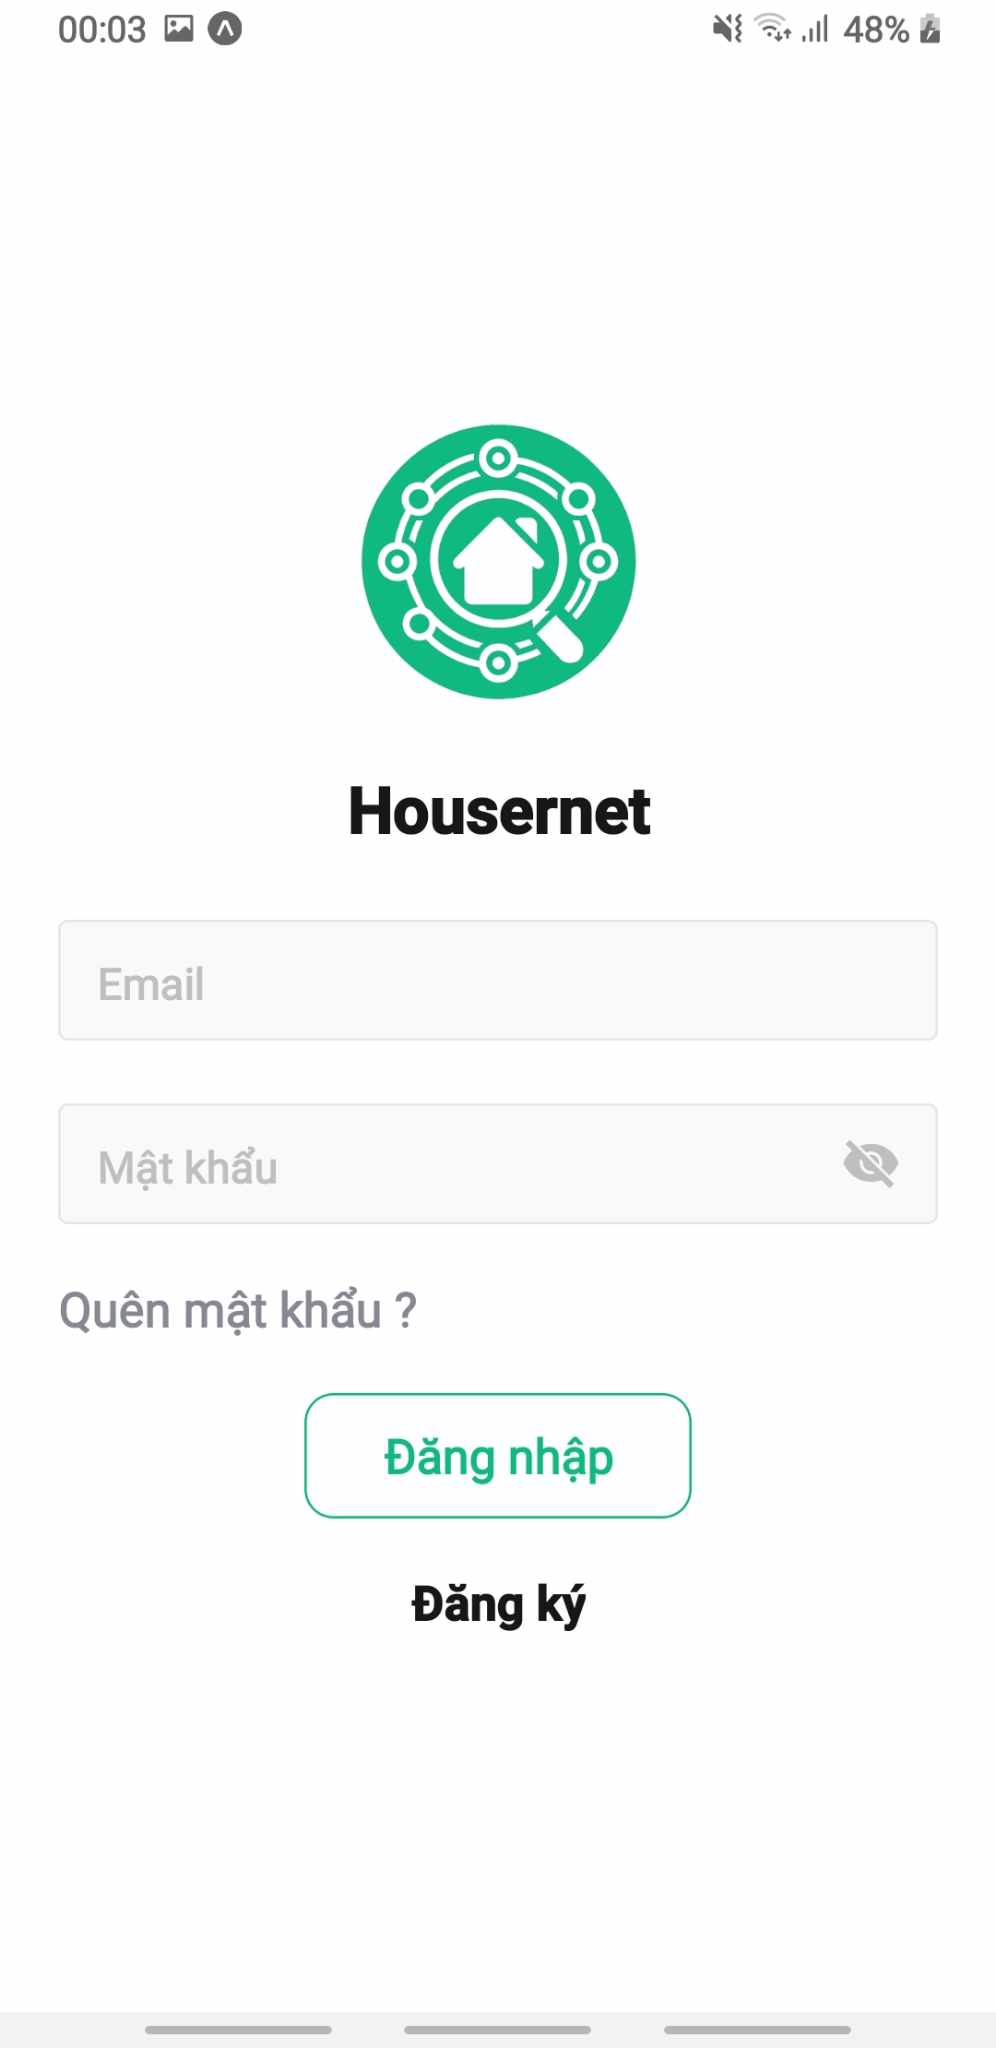
\includegraphics[width=0.5\textwidth]{Images/app_image/app_6.jpg}
    \caption{Đăng nhập}
\end{figure}
Đây là màn hình đầu tiên mà người dùng nhìn thấy khi mở ứng dụng, tại đây yêu cầu người dùng nhập username và password để tiến hành đăng nhập và sử dụng ứng dụng
\subsection{Đăng ký}
\begin{figure}[H]
    \centering
    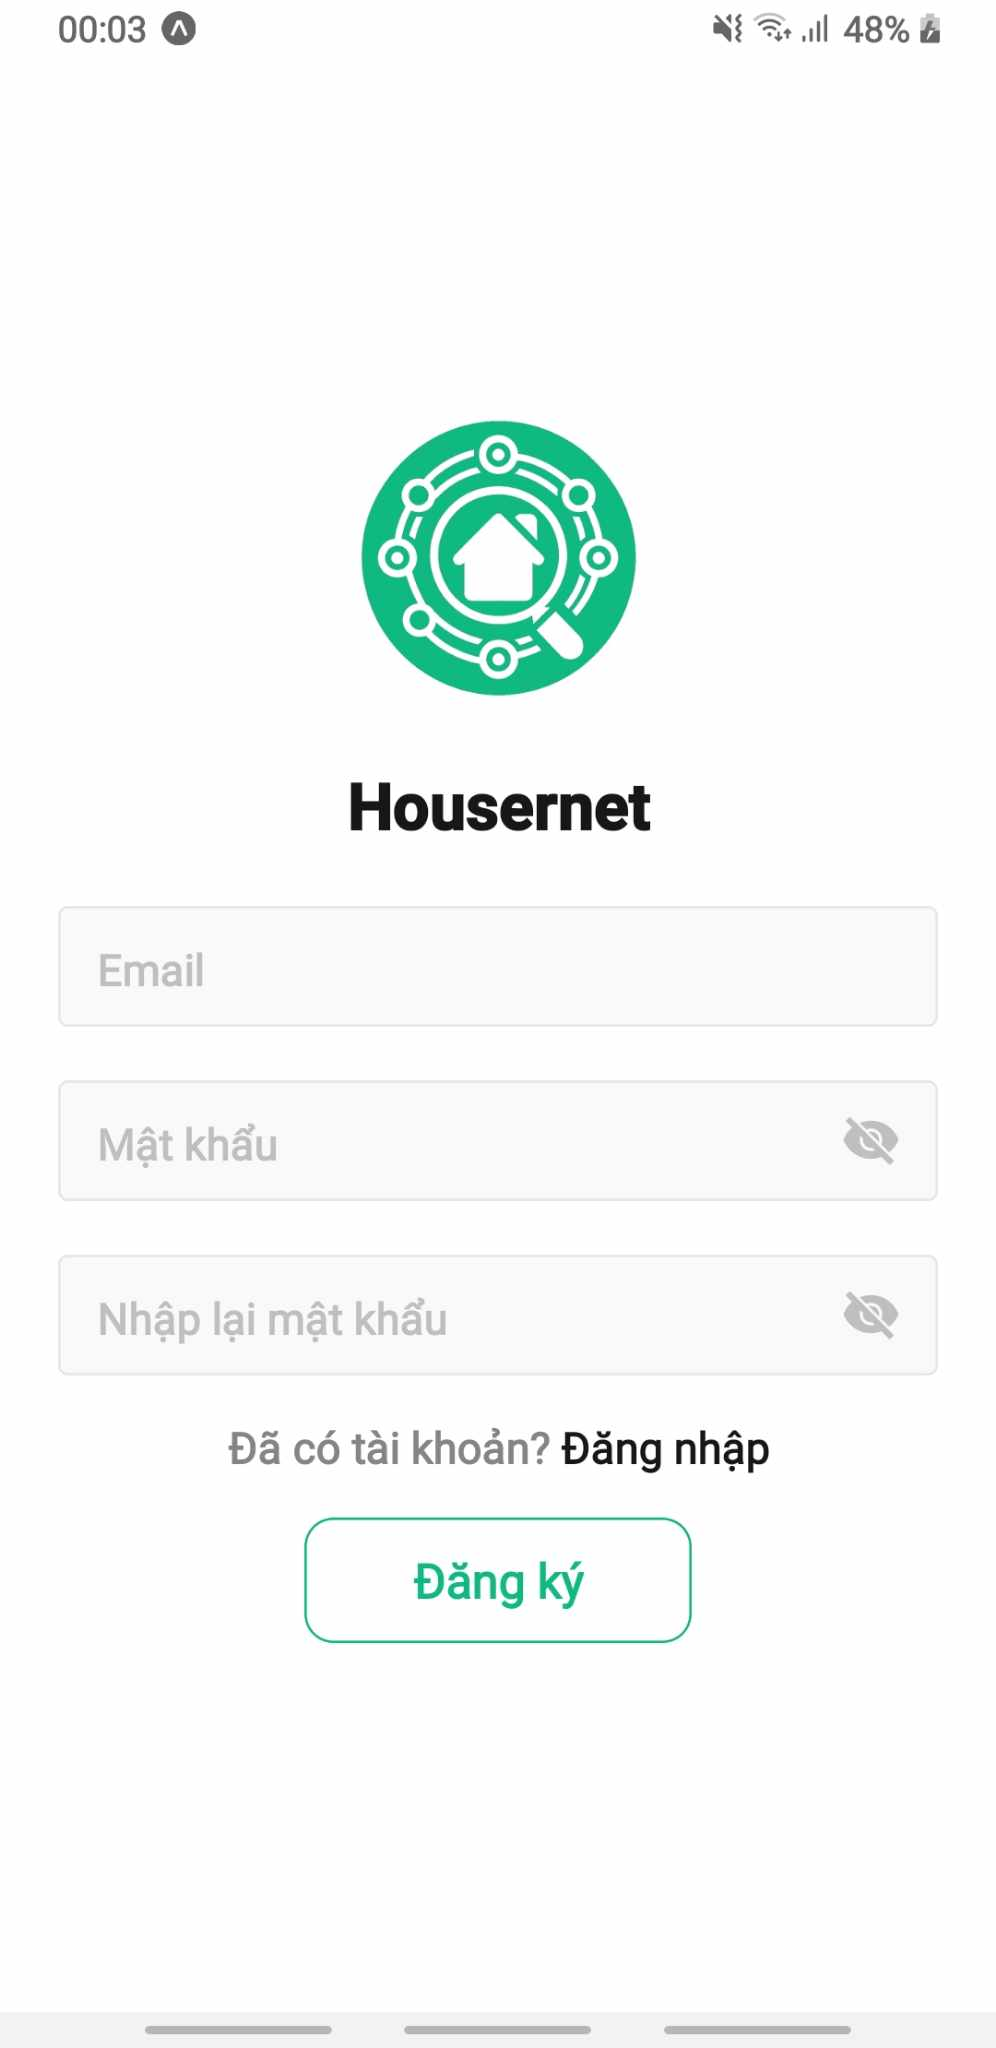
\includegraphics[width=0.5\textwidth]{Images/app_image/app_5.jpg}
    \caption{Đăng ký}
\end{figure}
Màn hình đăng ký được thiết kế để hỗ trợ những người dùng lần đầu tiên dùng app, người dùng tiến hành tạo tài khoản tại đây bằng cách thêm các thông tin về username và password là có thể sử dụng được app, những thông tin khác sẽ có thể bổ sung sau ở profile sau khi đăng nhập thành công
\subsection{Home}
\begin{figure}[H]
    \centering
    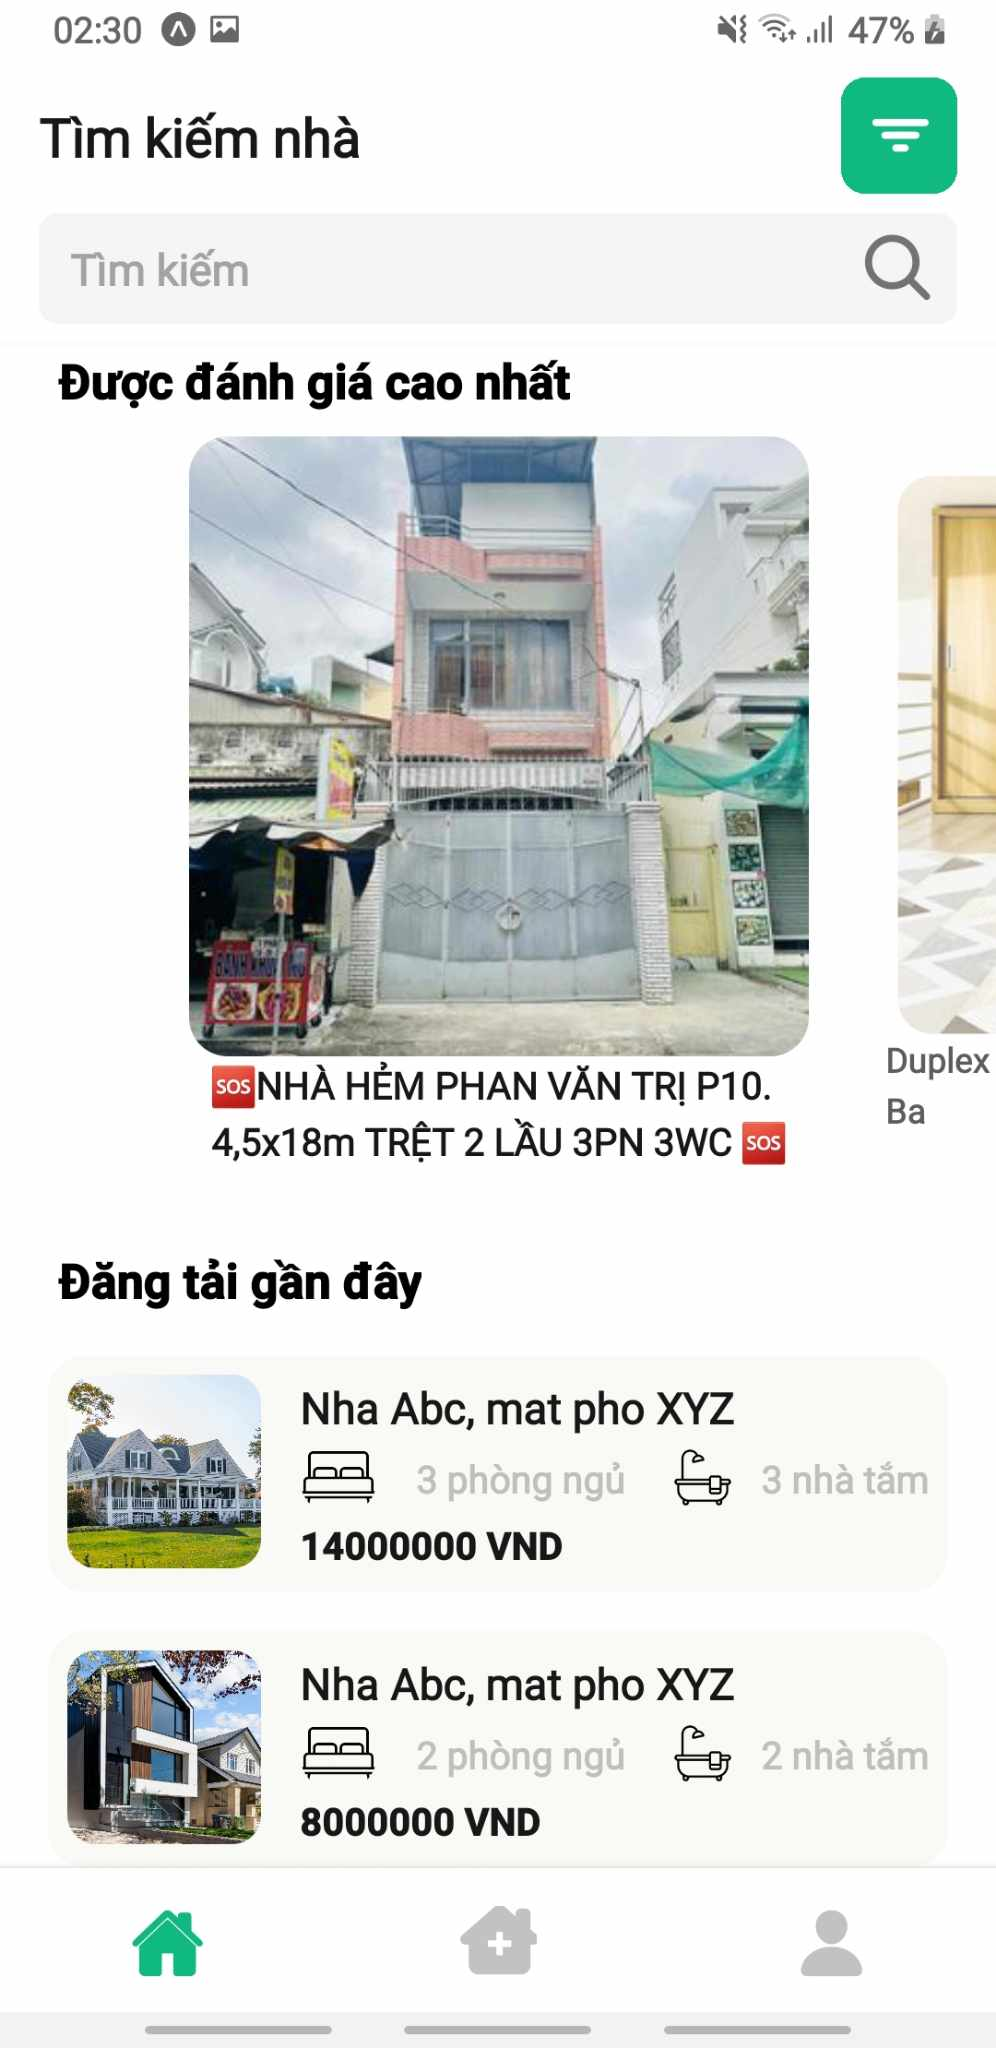
\includegraphics[width=0.5\textwidth]{Images/app_image/app_9.jpg}
    \caption{Trang chủ}
\end{figure}
Trang chủ của ứng dụng sẽ gồm các phần như sau :
\begin{itemize}
    \item Thanh search để người dùng có thể nhập câu search tìm nhà theo ý muốn
    \item Nút bộ lọc: để lọc kết quả theo các trường thông tin được cung cấp sẵn trong app
    \item Danh sách nhà trọ được đánh giá cao nhất
    \item Danh sách nhà trọ vừa được cập nhật
\end{itemize}
\subsection{Bộ lọc tìm kiếm}
\begin{figure}[H]
    \centering
    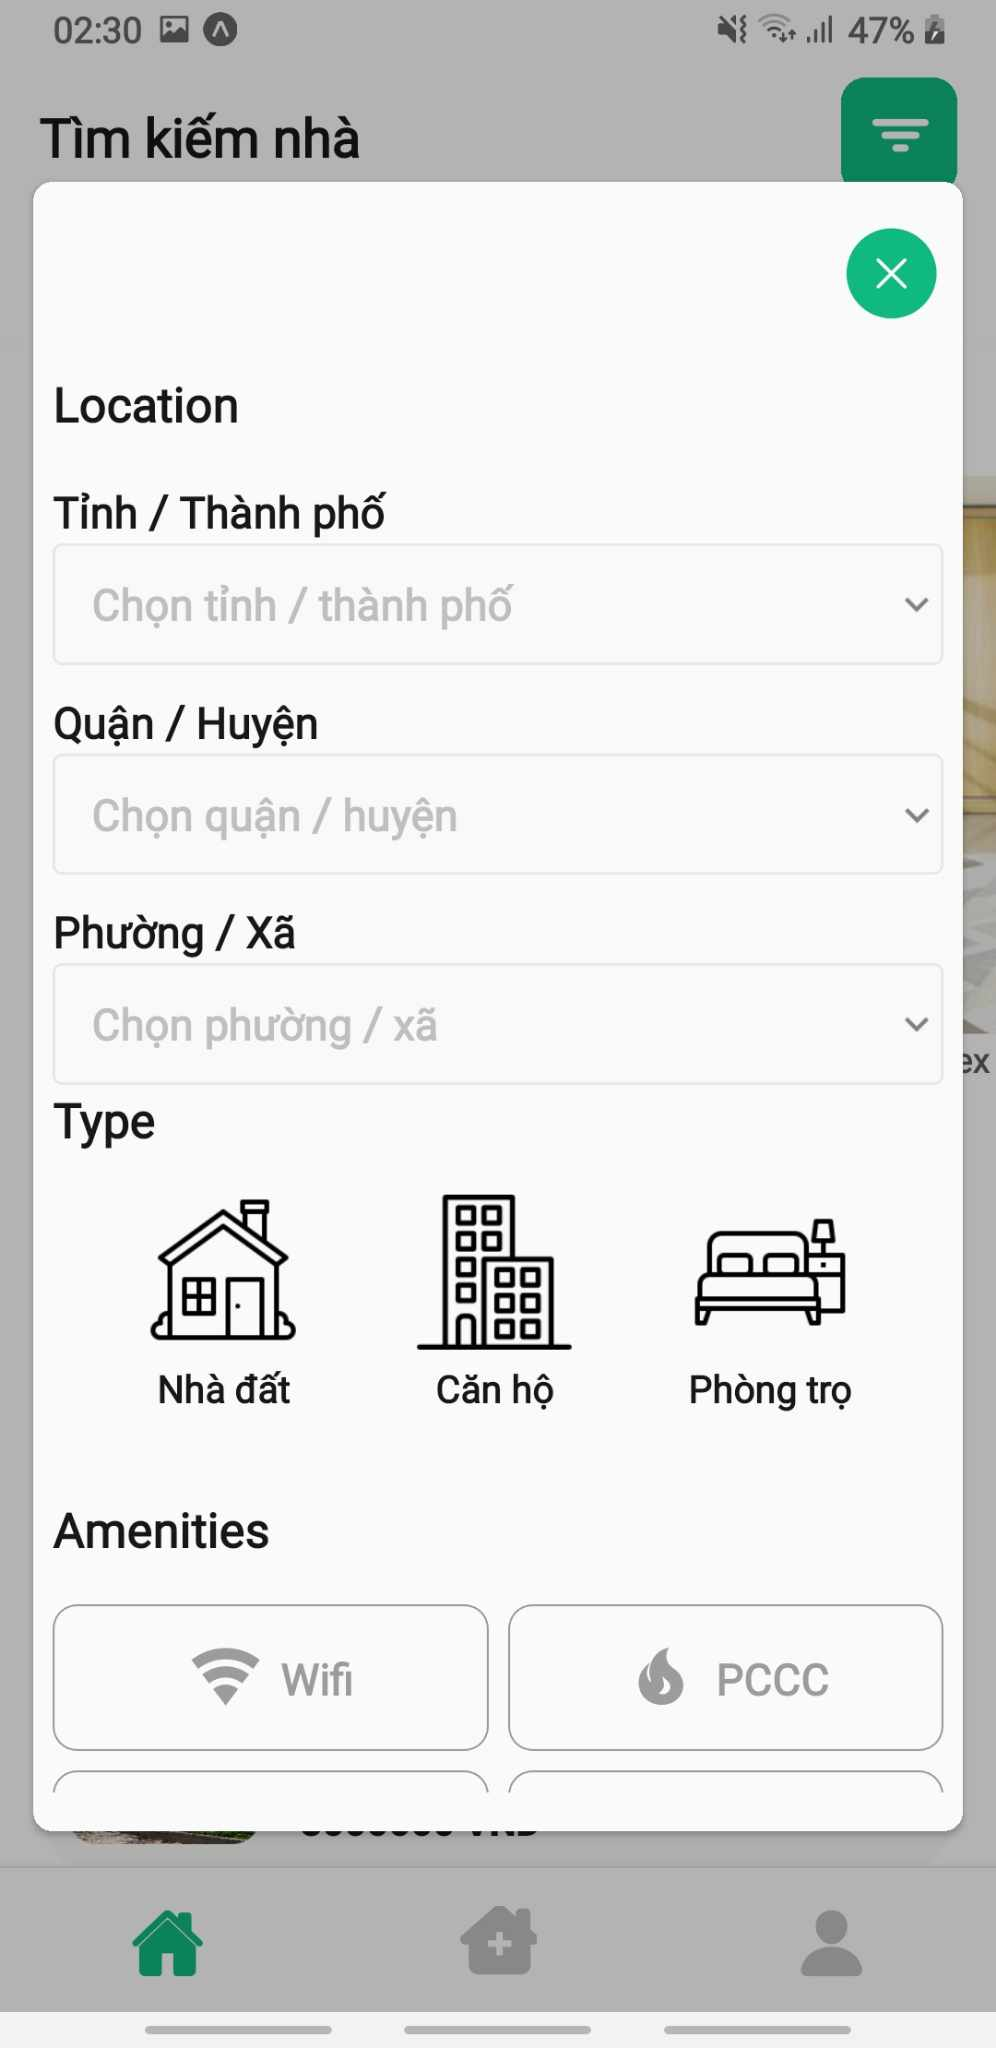
\includegraphics[width=0.5\textwidth]{Images/app_image/app_8.jpg}
    \caption{Bộ lọc tìm kiếm với các trường tìm kiếm theo loại nhà, địa chỉ, giá tiền}
\end{figure}
Bộ lọc tìm kiếm nhà dựa trên các trường thông tin đã được cung cấp trong ứng dụng, chỉ cần chọn rồi chọn filter sẽ ra được danh sách các nhà trùng khớp với thông tin cần filter. Ứng dụng sẽ lọc được các trường thông tin như sau
\begin{itemize}
    \item Địa điểm lọc theo tỉnh thành, quận/huyện và phường xã
    \item Loại nhà mong muốn gồm có : nhà đất, căn hộ, phòng trọ
    \item Các tiện ích như : camera an ninh, tủ lạnh, tv,...
    \item Khung giá tiền của nhà thuê
\end{itemize}
\subsection{Trang tìm kiếm}
\begin{figure}[H]
    \centering
    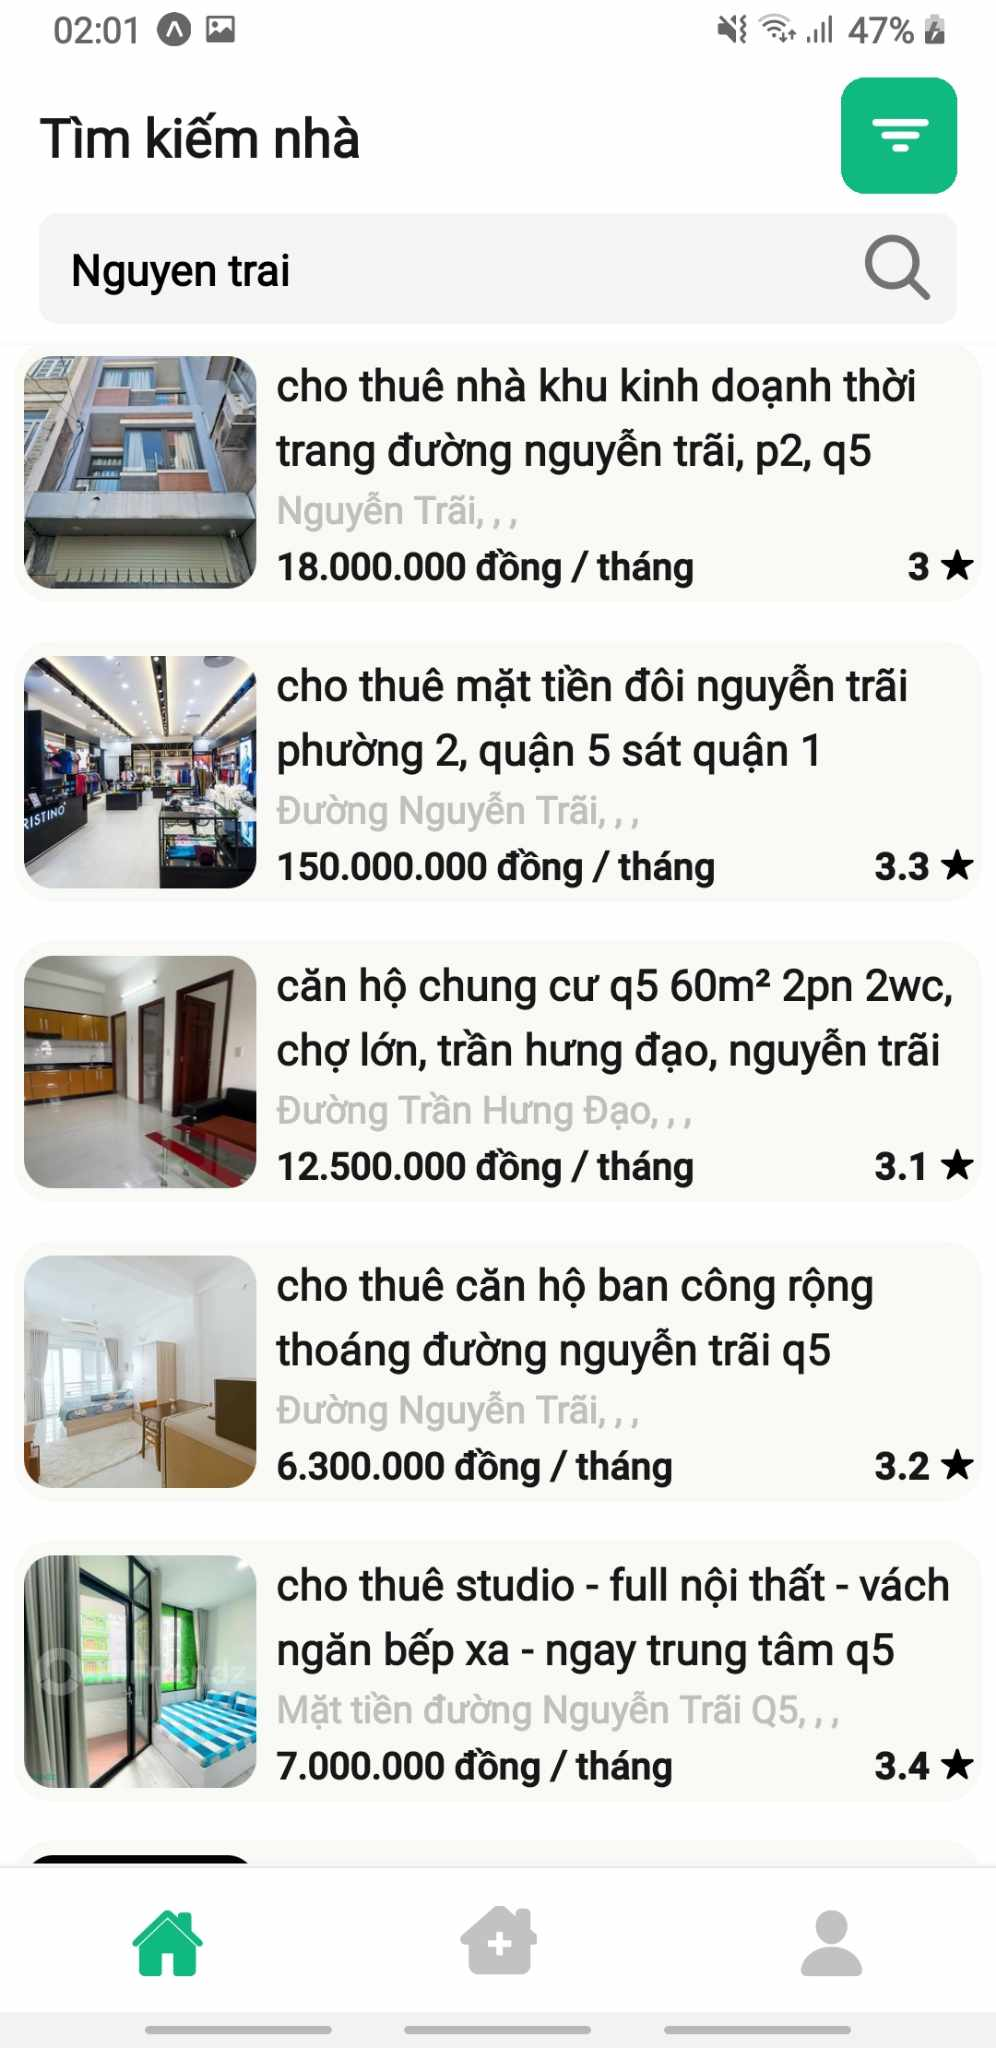
\includegraphics[width=0.5\textwidth]{Images/app_image/app_7.jpg}
    \caption{Trang tìm kiếm và kết quả trả về}
\end{figure}
Danh sách các nhà tìm được ứng với những từ khóa nhập vào trong thanh search sẽ cho ra, ví dụ ở hình trên khi nhập từ khóa \"Nguyen trai\", danh sách sẽ trả về danh sách các nhà có liên quan đến từ khóa "Nguyen trai" như nằm trên đường nguyễn trãi, hoặc nằm gần nguyễn 
\subsection{Trang chi tiết}
\begin{figure}[H]
    \centering
    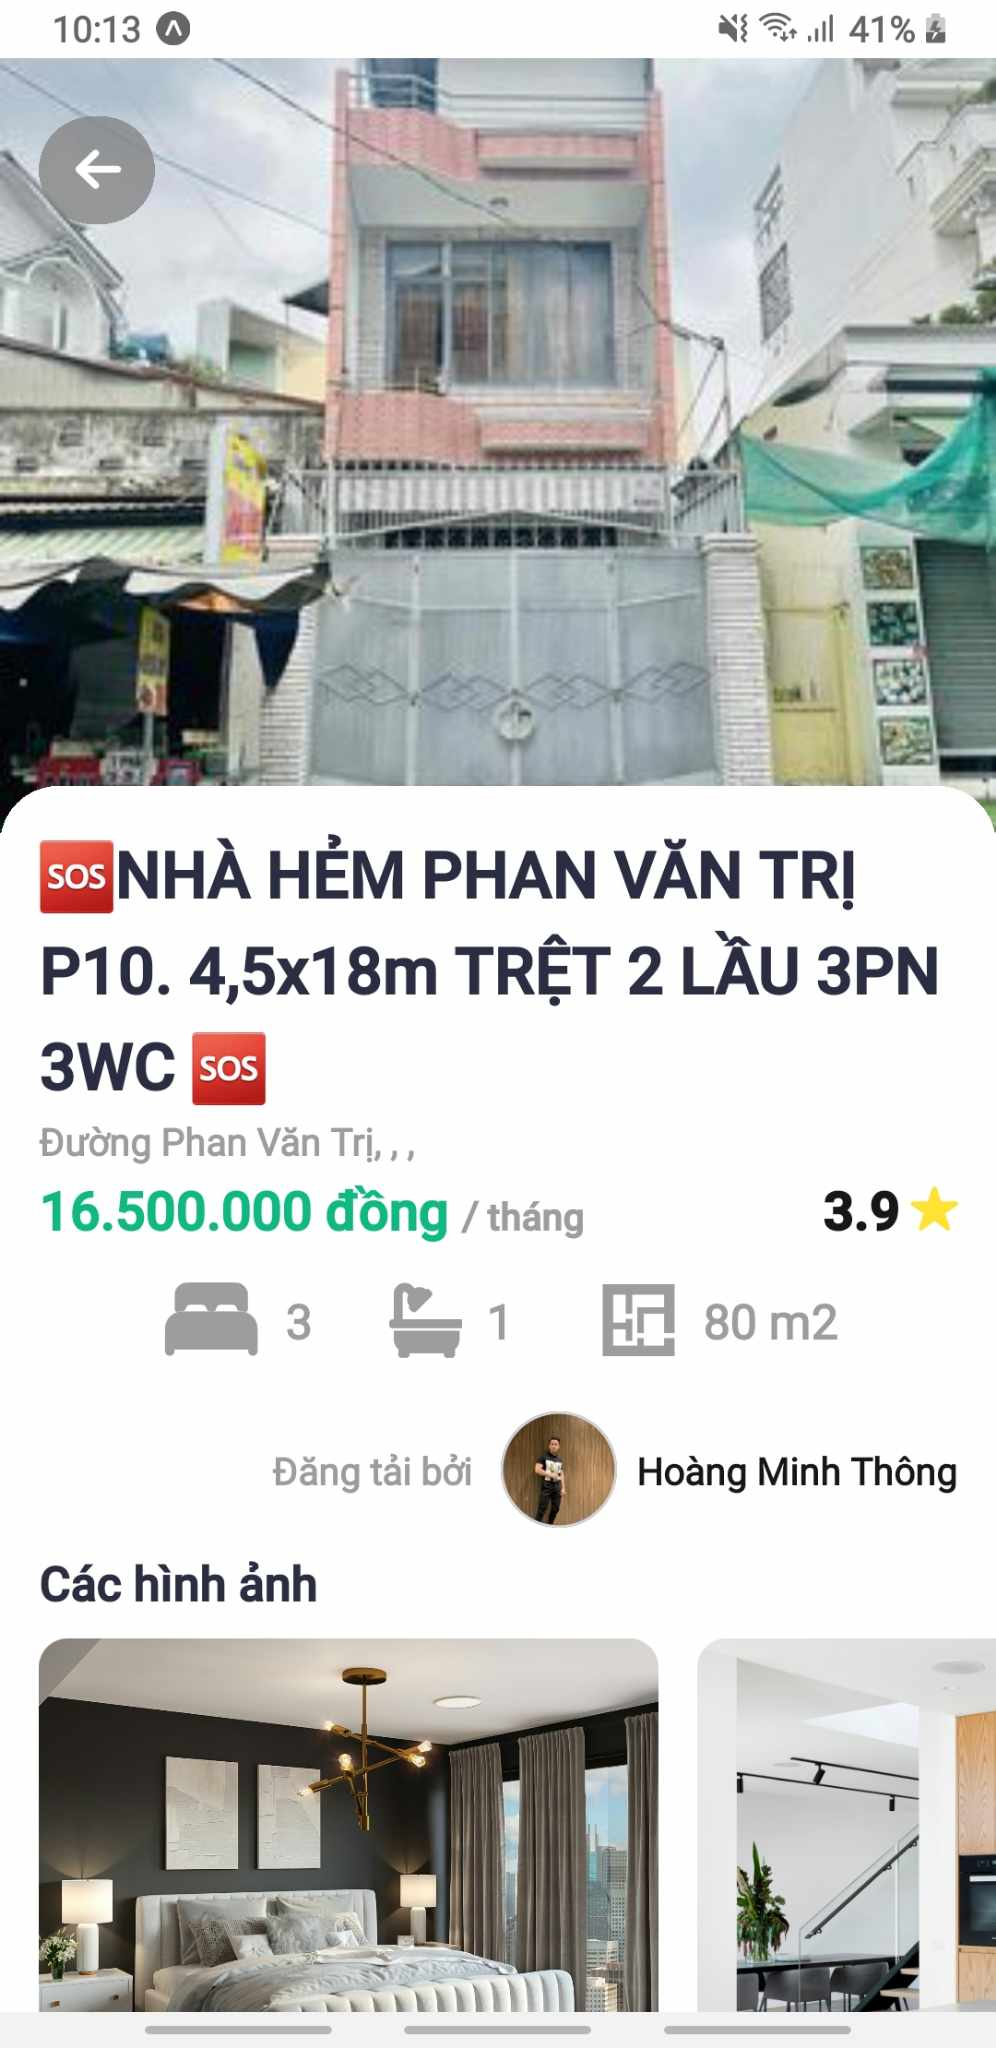
\includegraphics[width=0.5\textwidth]{Images/app_image/app_12.jpg}
    \caption{Trang chi tiết của từng nhà trọ}
\end{figure}
Trang chi tiết của từng nhà sẽ có các thông tin như tên, hình ảnh, địa điểm, chủ cho thuê,diện tích, số lượng các phòng, danh sách bình luận,...
\subsection{Bình luận}
\begin{figure}[H]
    \centering
    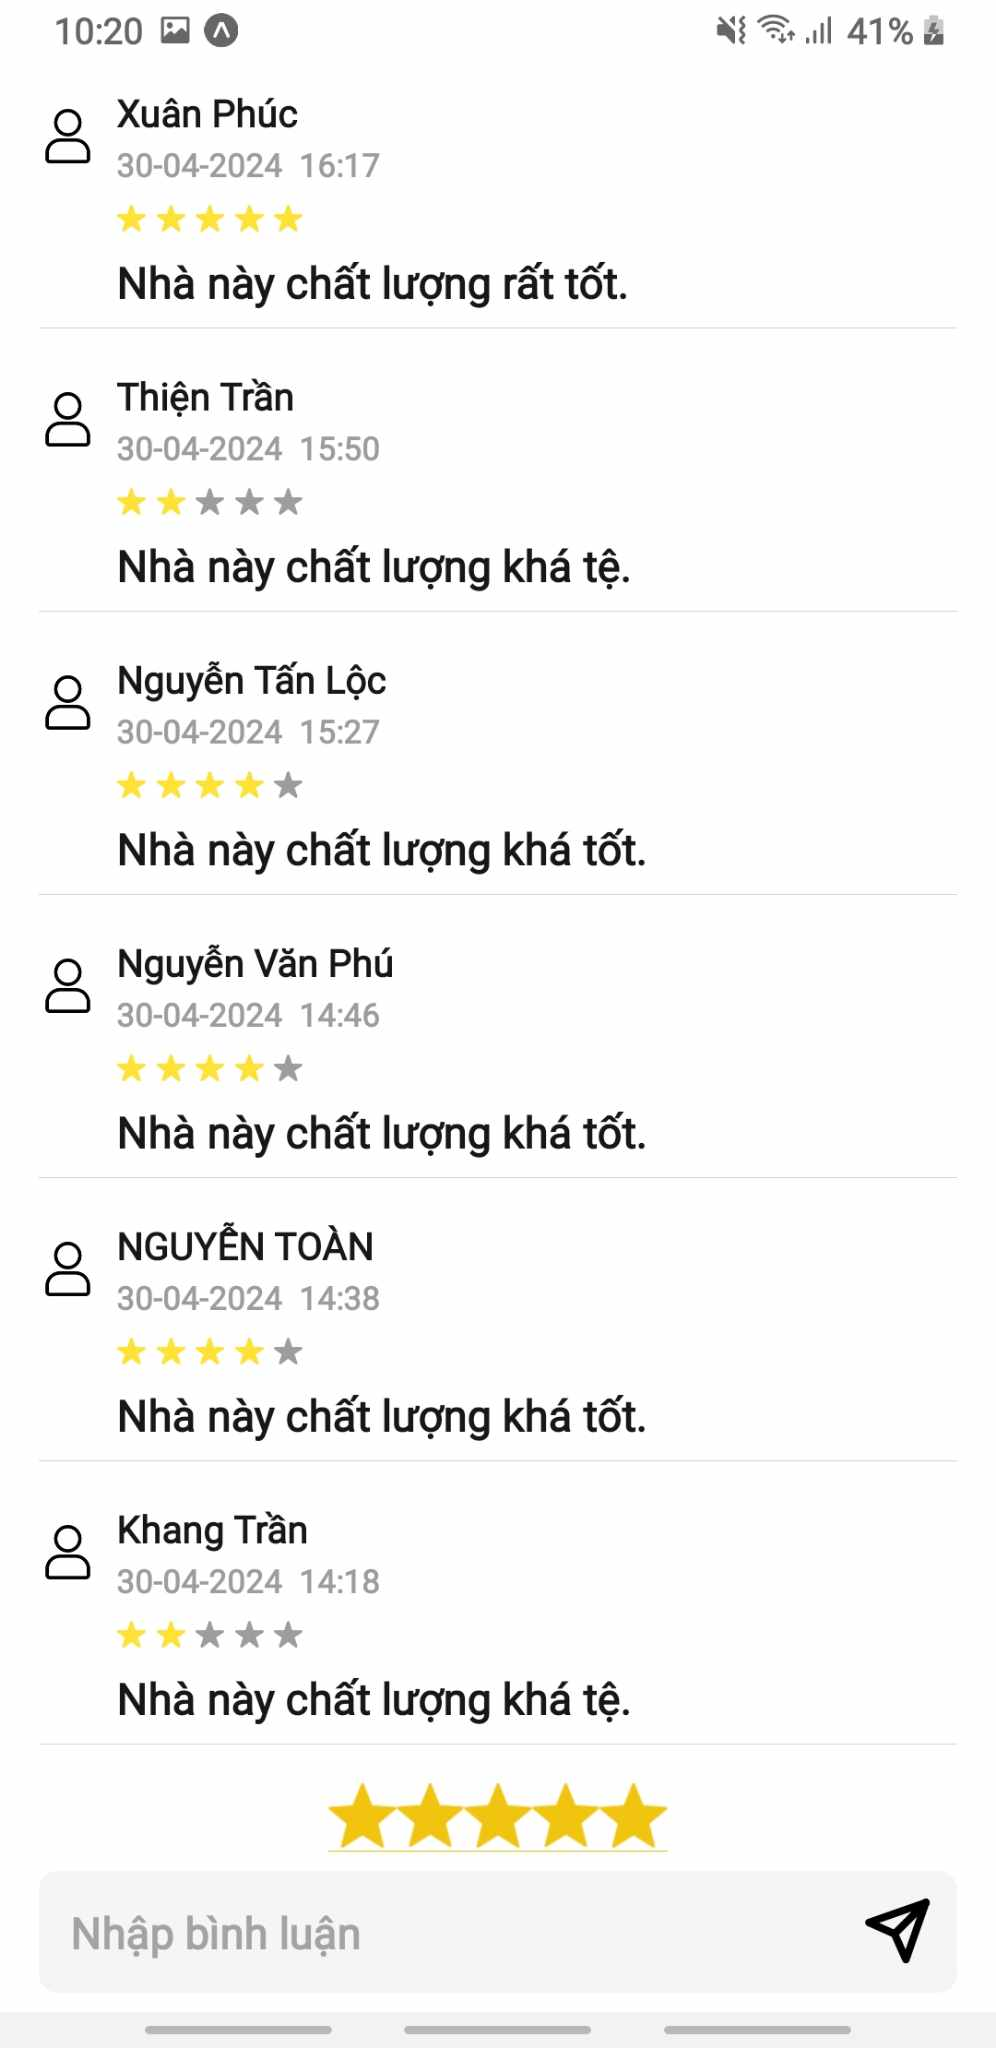
\includegraphics[width=0.5\textwidth]{Images/app_image/app_11.jpg}
    \caption{Danh sách bình luận trong từng nhà trọ tại trang chi tiết}
\end{figure}
Danh sách các bình luận trong đó mỗi bình luận bao gồm tên người dùng, đánh giá của họ với nhà
\subsection{Trang Profile}
\begin{figure}[H]
    \centering
    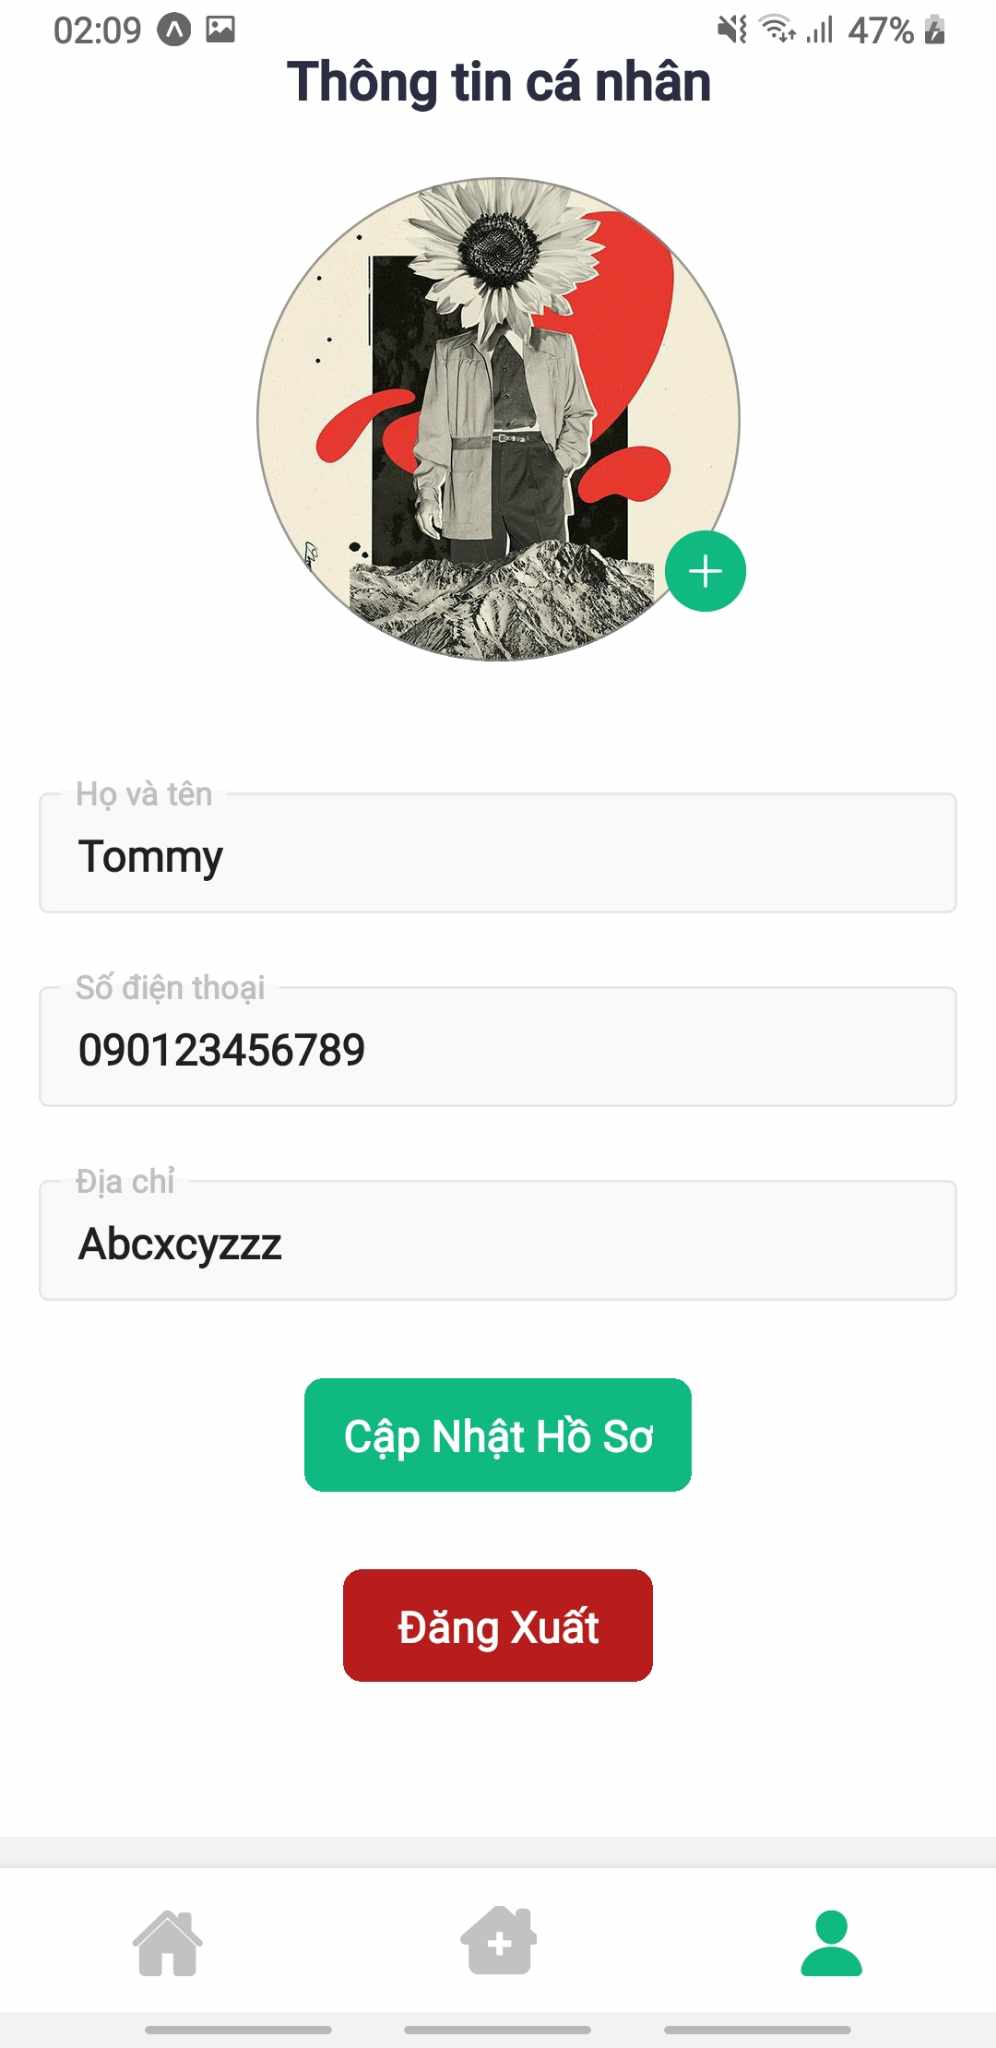
\includegraphics[width=0.5\textwidth]{Images/app_image/app_4.jpg}
    \caption{Trang profile thông tin của người dùng}
\end{figure}
\subsection{Danh sách nhà sỡ hữu}\begin{figure}[H]
    \centering
    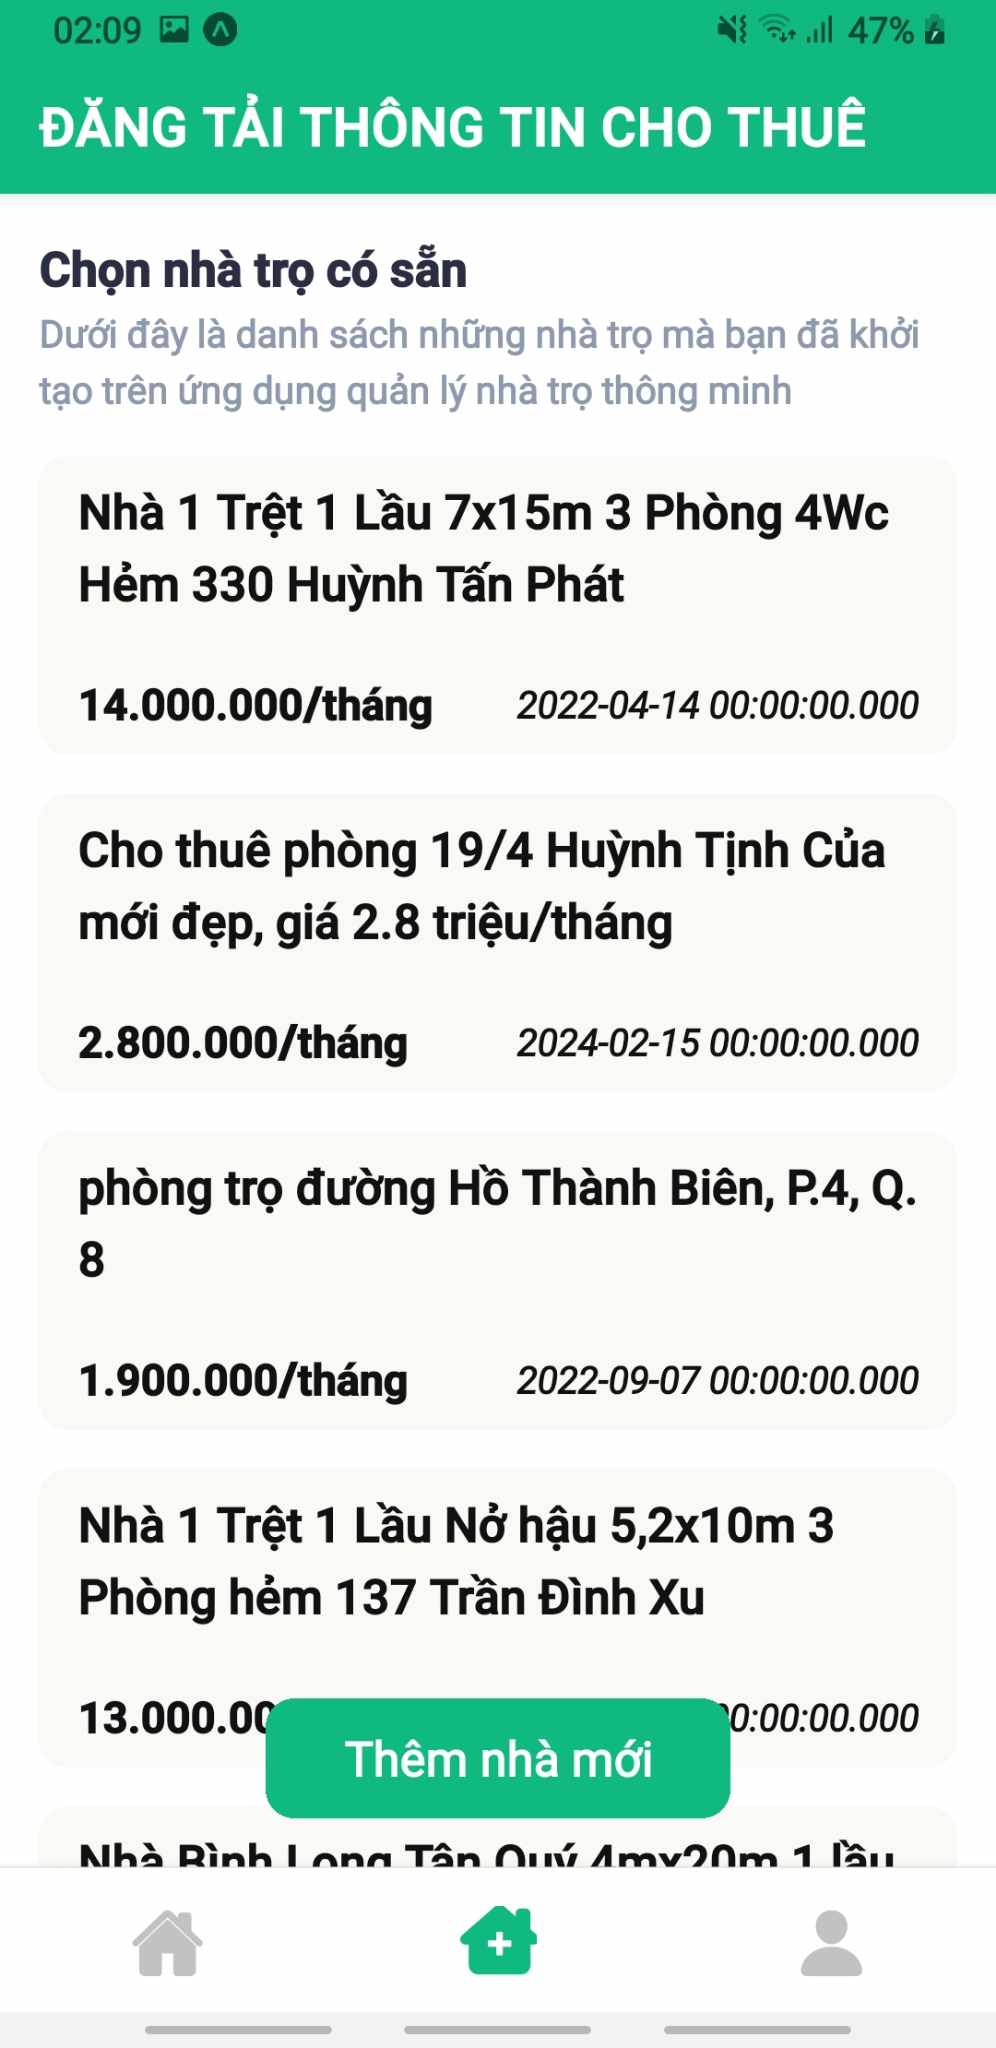
\includegraphics[width=0.5\textwidth]{Images/app_image/app_3.jpg}
    \caption{Danh sách nhà mà người dùng sở hữu}
\end{figure}
Danh sách các nhà do người dùng đó sở hữu, khi chọn một nhà bất kỳ sẽ hiện lên một tab gồm các chức năng như
\begin{itemize}
    \item Không chọn nhà đó nữa
    \item Xem chi tiết
    \item Chỉnh sửa
    \item Xóa
\end{itemize}
\subsection{Đăng tải nhà mới}
\begin{figure}[H]
    \centering
    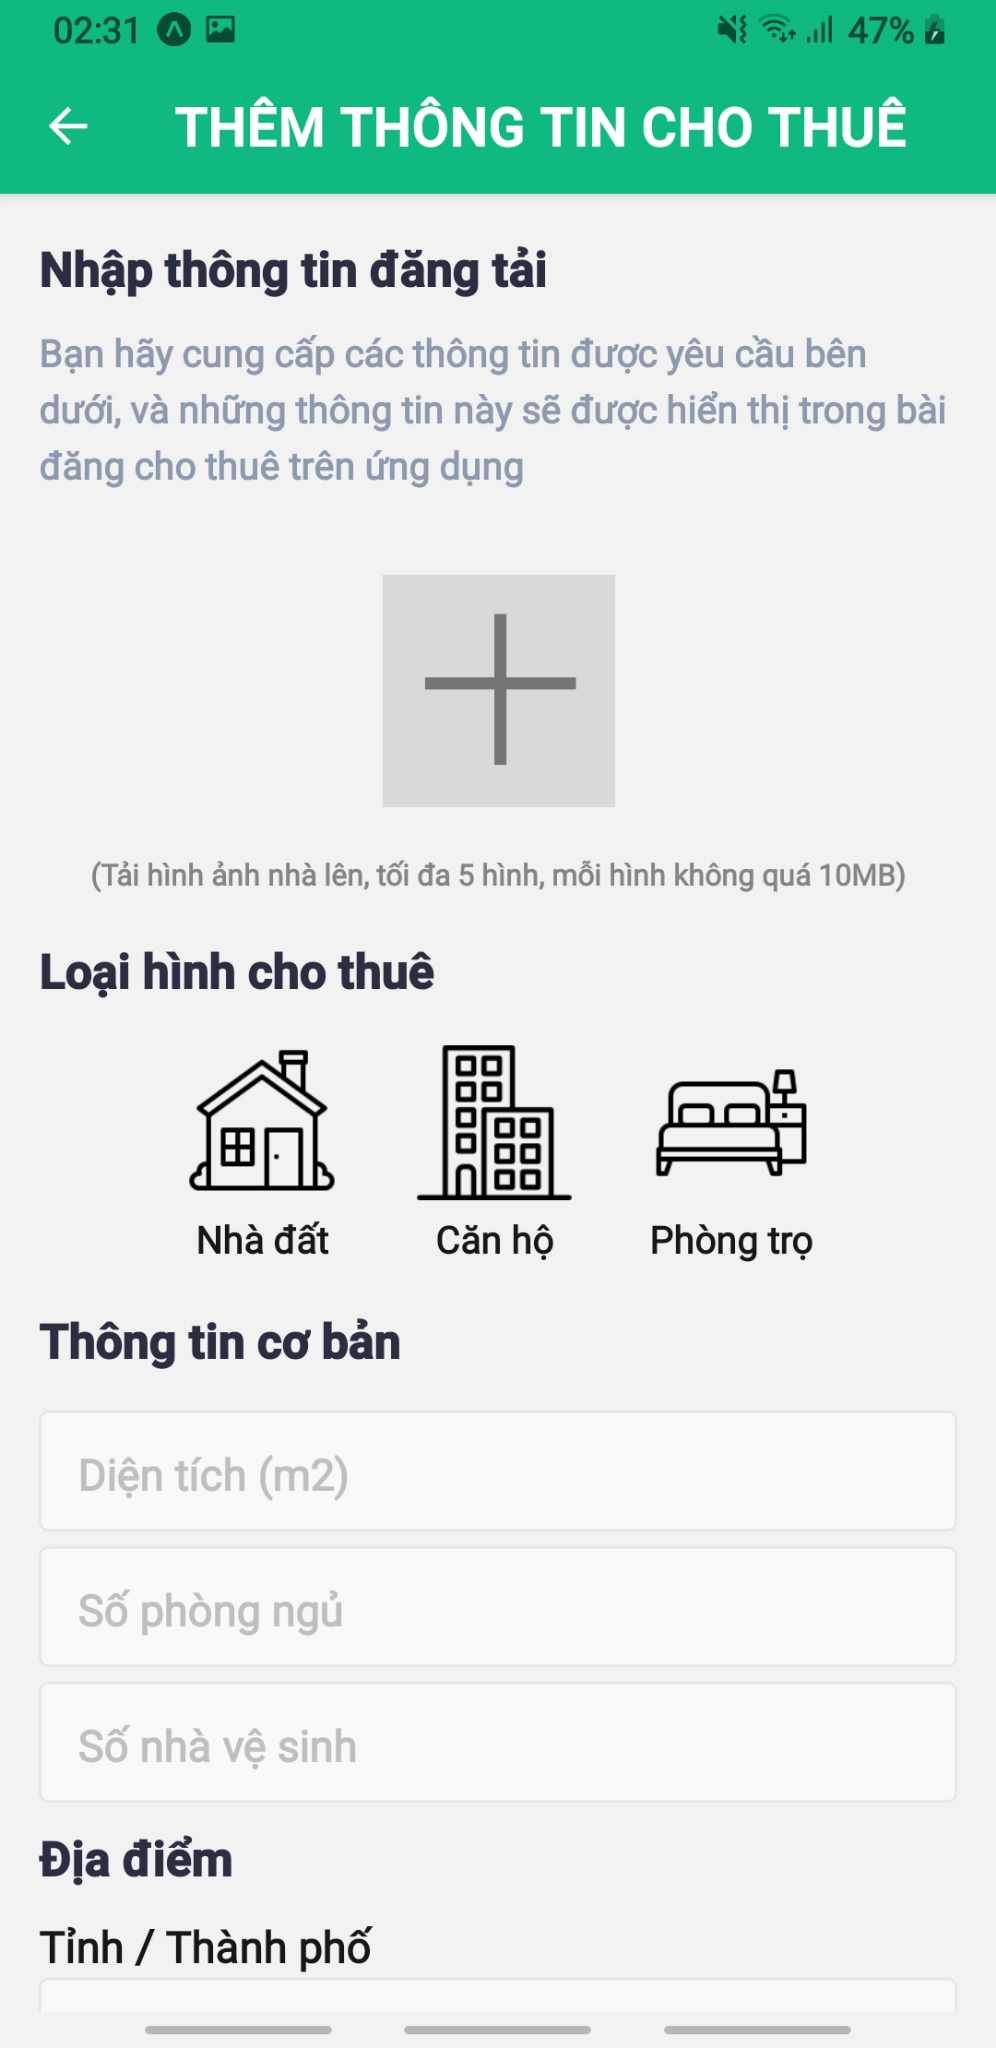
\includegraphics[width=0.5\textwidth]{Images/app_image/app_10.jpg}
    \caption{Đăng tải nhà mới}
\end{figure}
Đăng tải nhà mới lên ứng dụng , người dùng sẽ nhập những thông tin mới thêm hình ảnh, chọn loại hình cho thuê, diện tích, số phòng ngủ, vệ sinh và địa điểm
\subsection{Chỉnh sửa nhà trọ}
\begin{figure}[H]
    \centering
    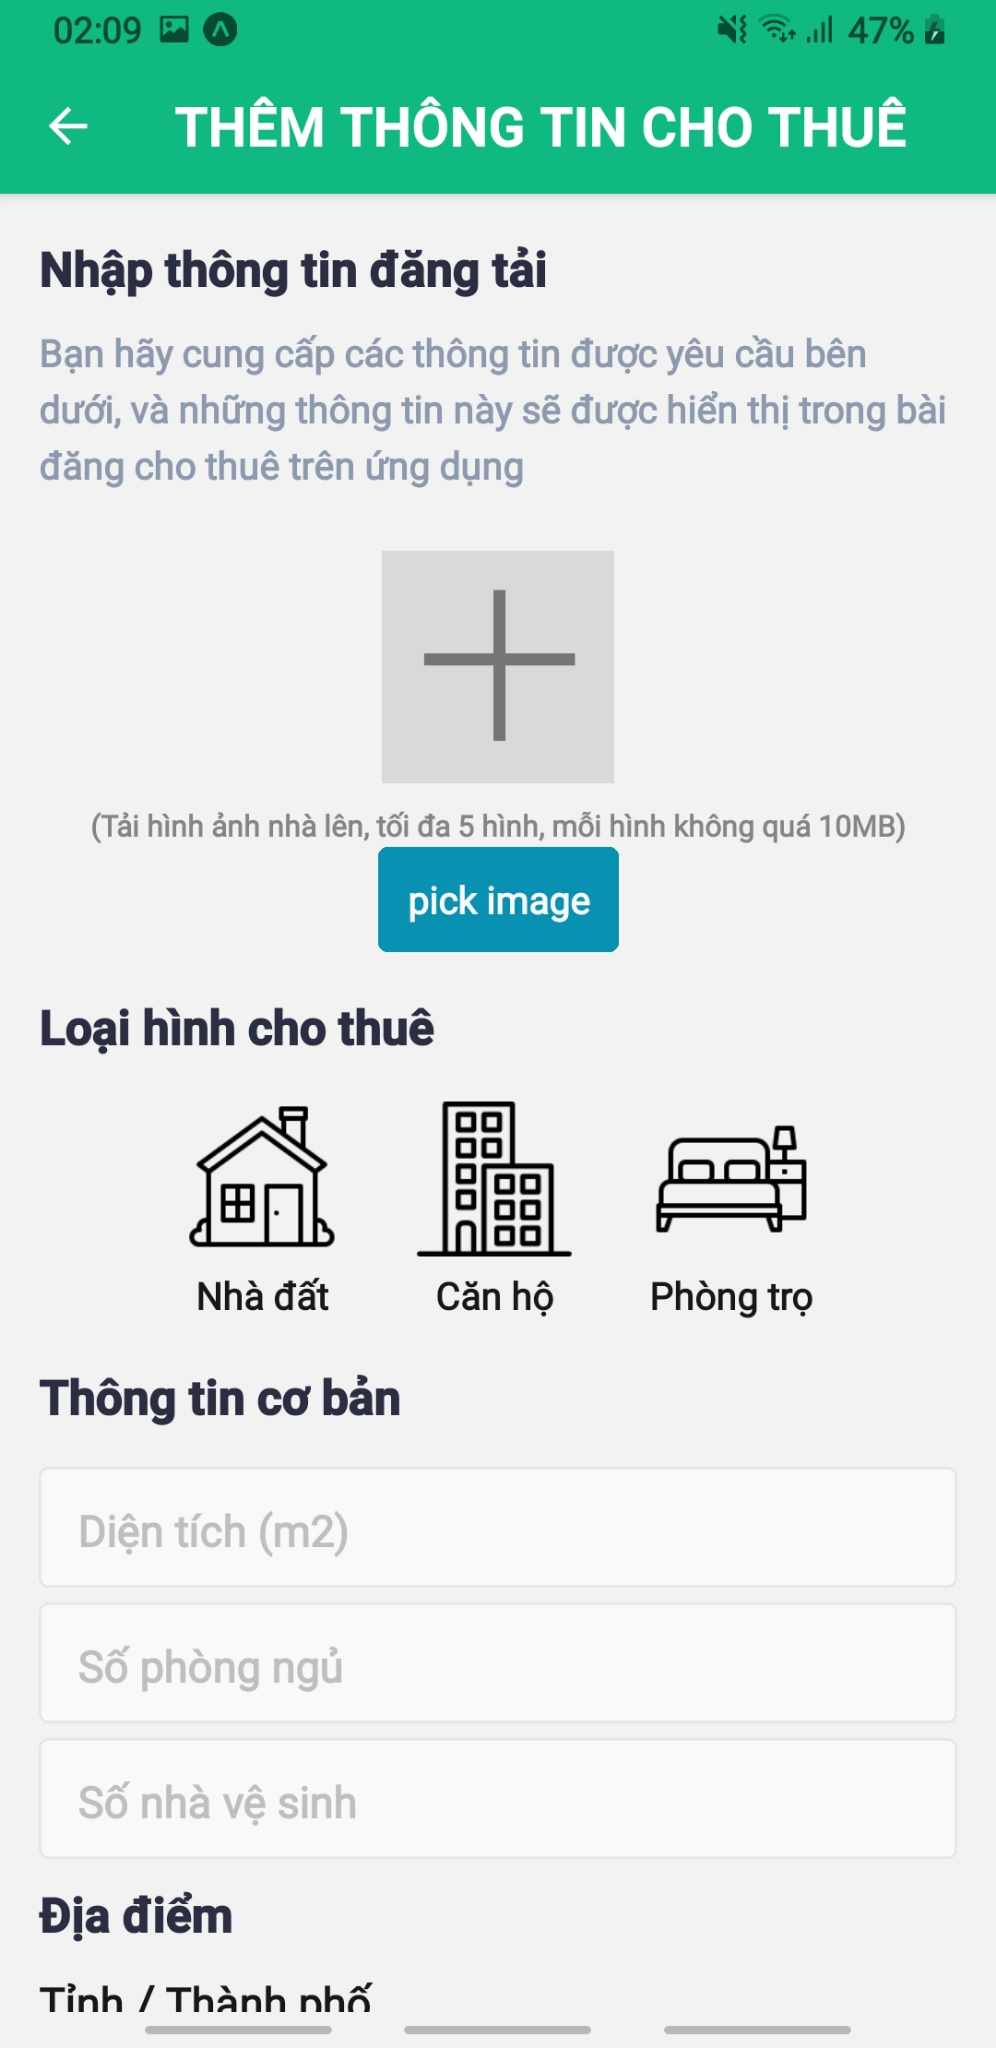
\includegraphics[width=0.5\textwidth]{Images/app_image/app_2.jpg}
    \caption{Chỉnh sửa nhà trong danh sách các nhà trọ}
\end{figure}
Tương tự như đăng nhà mới, cũng có các trường thông tin có sẵn
\subsection{Xóa nhà sỡ hữu}
\begin{figure}[H]
    \centering
    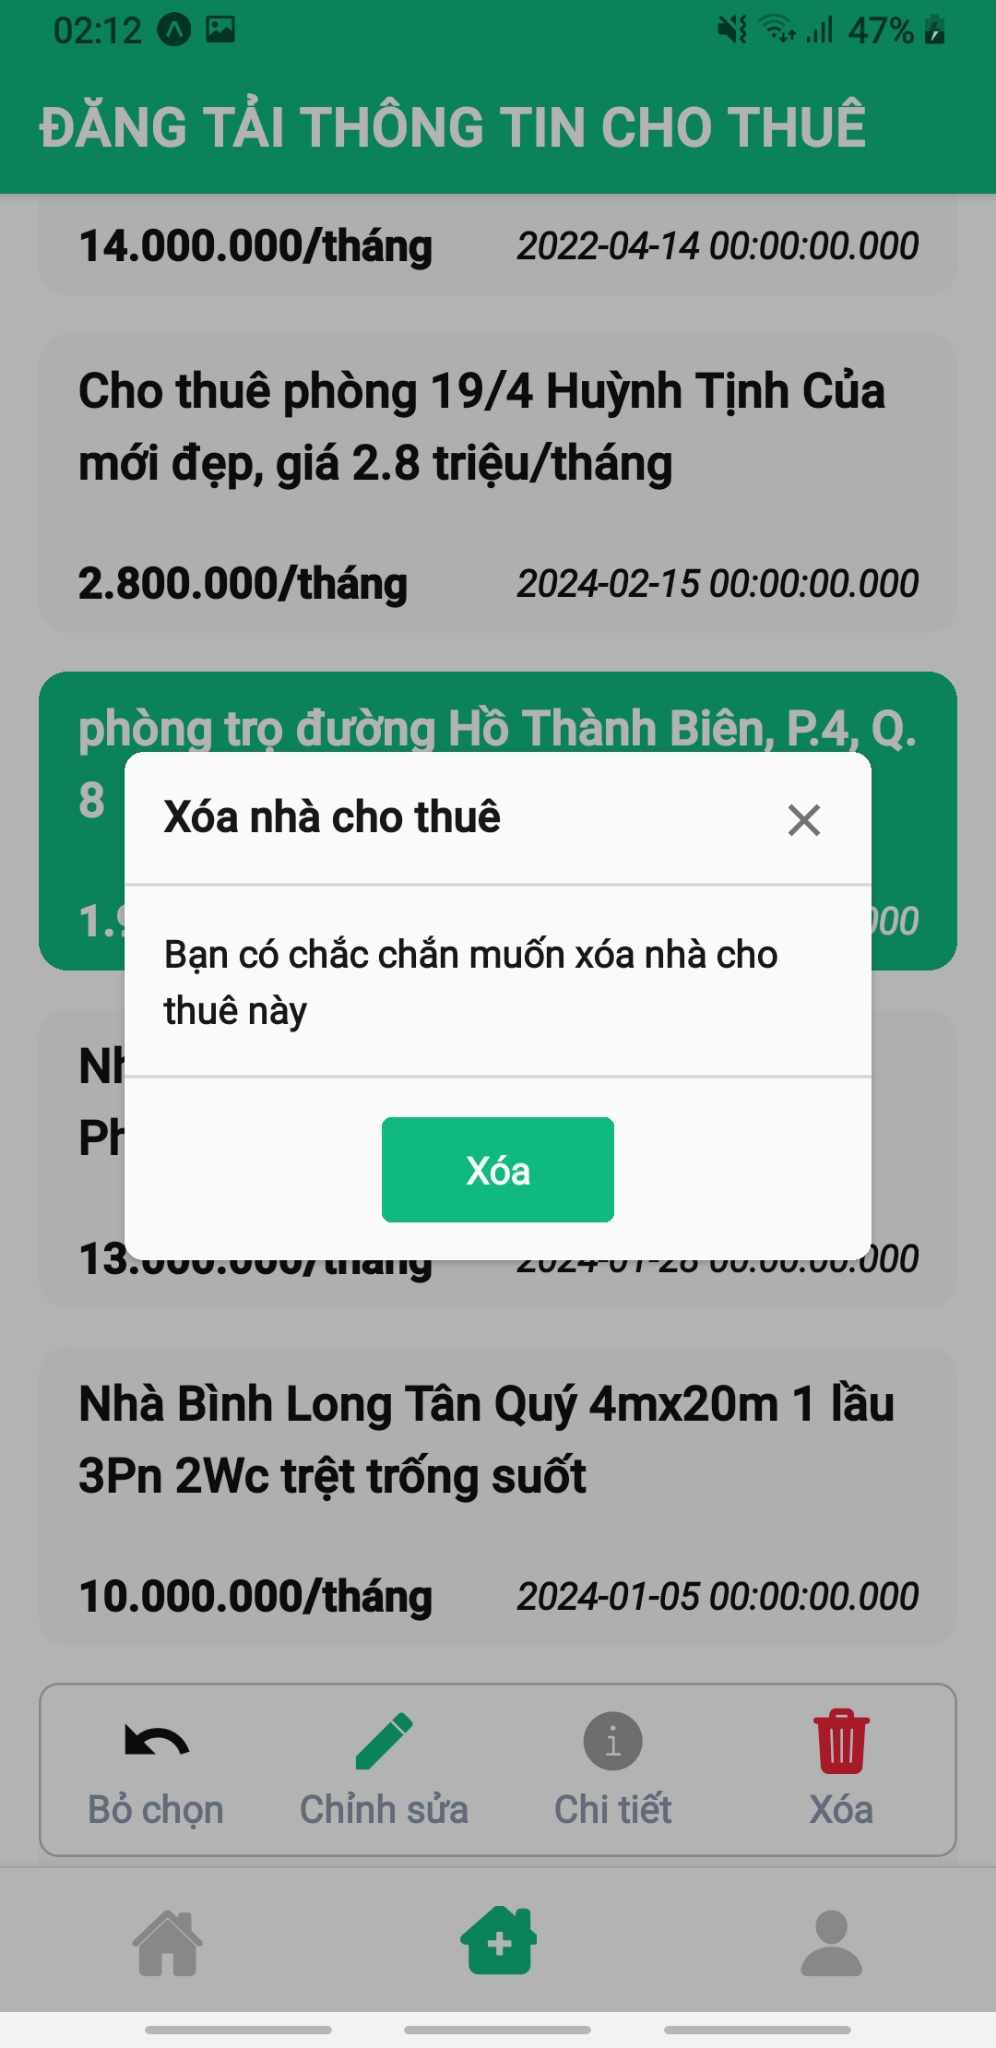
\includegraphics[width=0.5\textwidth]{Images/app_image/app_1.jpg}
    \caption{Xóa nhà trong danh sách nhà trọ}
\end{figure}
Khi chọn nhà cho thuê, ứng dụng sẽ hiển thị lên option để xóa, chọn xóa sẽ hiện lên một thông báo như hình, sau khi chọn xóa, nhà sẽ được xóa khỏi ứng dụng
\newpage

